% FUNDAMENTAÇÃO TEÓRICA--------------------------------------------------------

\chapter{FUNDAMENTAÇÃO TEÓRICA}
\label{chap:fundamentacao-teorica}

Este capítulo descreve as tecnologias e conceitos centrais utilizados durante a
concepção do projeto. As definições apresentadas são embasadas no material bibliográfico
revisado, que serviu de apoio no desenvolvimento de um trabalho fundamentado nas teorias
existentes.

\section{Raspberry Pi}
\label{sec:raspi}

O Raspberry Pi é uma família de computadores em placa única (SOC em inglês), com o tamanho de um cartão de crédito. Inicialmente seu objetivo era promover o ensino de computação (programação) básica em escolas, principalmente públicas, de todo o mundo. Entretanto, por possuir poder computacional razoável, uma boa quantidade de memória ram (a partir do modelo B) e um preço relativamente baixo, passou a ser usado para outros objetivos como: console de videogame clássico (emulação de jogos), gerencia de mídia (vídeos, fotos e musicas), estudos em eletrônica, domótica (automação residencial), internet das coisas e robótica. \citeonline{jucapereira2018aplicacoes} \par
Uma versão do sistema operacional Debian Linux, chamada Raspbian, foi criada para o Raspberry Pi, portando também uma serie de aplicativos e ferramentas de desenvolvimentos já existentes para computadores da plataforma PC. Dessa modo, o desenvolvimento de programas se torna uma tarefa extremamente simples, já que o hardware é abstraído pelo sistema operacional, e não é necessário conhecimento especifico do hardware do Raspberry Pi (plataforma ARM). As linguagens mais utilizadas para desenvolvimento de software com bibliotecas disponíveis para interação com o hardware são o C/C++ e Python, porém, é possível desenvolver em outras linguagens de programação como o PHP e Java. \citeonline{jucapereira2018aplicacoes} \par

\begin{figure}[H]
	\centering
	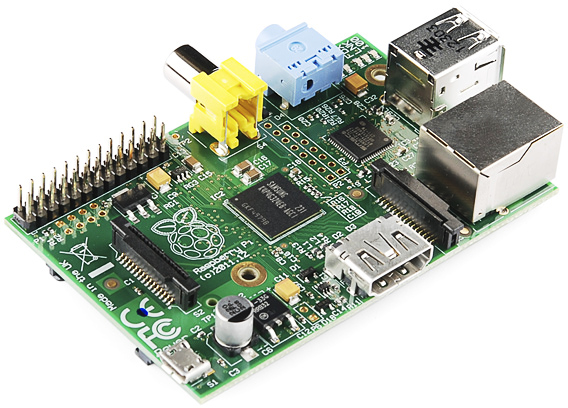
\includegraphics[width=0.6\textwidth]{figuras/raspberrypi_model_b.jpg}
	\caption{Raspberry Pi (Modelo B).}
	\fonte{ \citeonline{sparkfun2019}}
	\label{fig:raspi_modelb}
\end{figure}

\section{Servo Motor}
\label{sec:servomotor}

Um servo motor, visto na \autoref{fig:servo_g9}, é um atuador rotatório, ou atuador linear, que permite um controle preciso da posição linear ou angular, velocidade e aceleração de uma carga ligada ao seu eixo. Consiste basicamente em um motor de corrente continua (para o caso particular desse trabalho), acoplado a um sensor (potenciômetro), como ilustrado na \autoref{fig:insideaservo}, para ler sua posição durante o movimento. Normalmente, os motores servos necessitam de um sinal de controle modulado por largura de pulso (PWM em ingles) para operar. \citeonline{petruzella2009electric} \par

\begin{figure}[h]
	\centering
	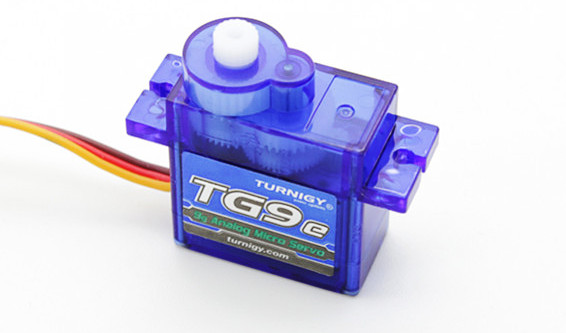
\includegraphics[width=0.6\textwidth]{figuras/servo_g9.jpg}
	\caption{Servo Micro TG9.}
	\fonte{ \citeonline{hobbyking2019}}
	\label{fig:servo_g9}
\end{figure}

O servo motor opera em malha fechada, isto é, seu controlador compara a velocidade de movimento e sua posição para gerar o próximo comando de movimento, minimizando o erro. \citeonline{petruzella2009electric} O esquema de funcionamento do servo motor é mostrado na figura \autoref{fig:servo_closed_loop}. 

\begin{figure}[h]
	\centering
	\begin{subfigure}{.5\textwidth}
		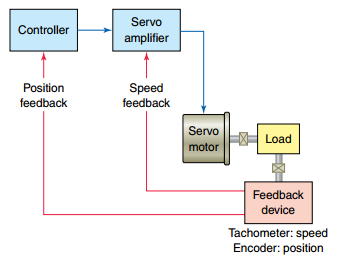
\includegraphics[width=0.95\textwidth]{figuras/servo_closed_loop.png}
		\caption{Sistema em malha fechada.}
		\fonte{ \citeonline{petruzella2009electric}}
		\label{fig:servo_closed_loop}
	\end{subfigure}%
	\begin{subfigure}{.5\textwidth}
		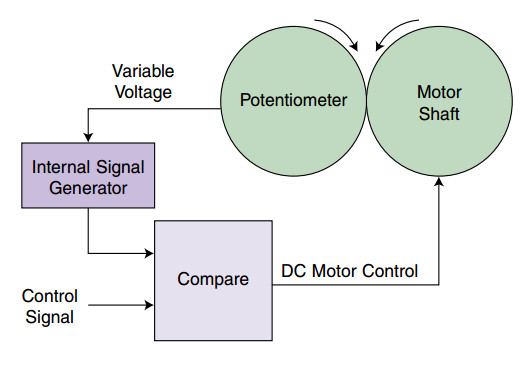
\includegraphics[width=0.95\textwidth]{figuras/inside_a_servo.jpg}
		\caption{Componentes internos.}
		\fonte{\citeonline{pinckney2006pulse}.}
		\label{fig:insideaservo}
	\end{subfigure}
	\caption{Sistema de controle de um servo motor.}
\end{figure}

\section{Modulação por Largura de Pulso}
\label{sec:pwm}

A modulação por largura de pulso é uma técnica empregada em diversas áreas da eletrônica, sendo utilizada para controlar fontes chaveadas, velocidade de motores, luminosidade, servo motores e diversas outras aplicações. Consiste em variar a o tempo em que um pulso de tensão oscila entre os níveis alto e baixo numa taxa rápida o suficiente para que a média dos pulsos crie um valor médio de tensão efetivo, ilustrado na \autoref{fig:pwm}. Ao valor definido pela divisão entre: a largura de pulso com a tensão em nível alto, e o período do sinal; é dado o nome ciclo de trabalho ou \textit{dutty cycle}. Variar o \textit{dutty cycle} significa variar a tensão média, isto é, a potência é proporcional a tensão média resultante. \citeonline{pinckney2006pulse}.

\begin{figure}[h]
	\centering
	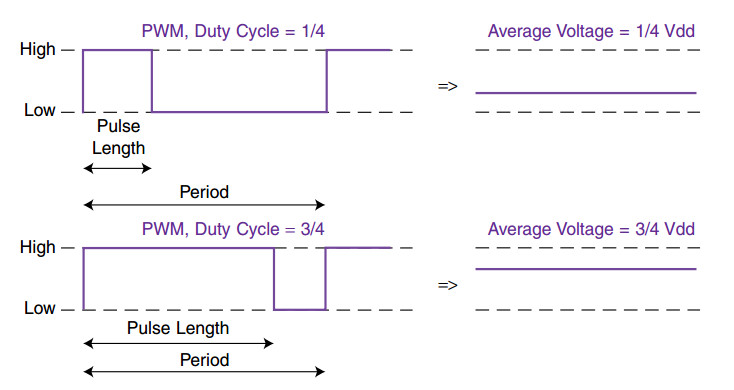
\includegraphics[width=1\textwidth]{figuras/pwm.jpg}
	\caption{Modulação por largura de pulso e tensão média resultante}
	\fonte{ \citeonline{pinckney2006pulse}}
	\label{fig:pwm}
\end{figure}

A largura de pulso pode ser calculada usando a equação \autoref{eq:duttycicle}.

\begin{equation}
{Dutty Cycle} = 100 \times \frac{Largura do Pulso}{Período}  
\label{eq:duttycicle}
\end{equation}

Onde: Duty Cycle é um valor dado em porcento, Largura do pulso e Período são valores dados em segundos.\par

Uma vez calculado o ciclo de trabalho, é possível calcular o valor da tensão média gerada pelo sinal através da \autoref{eq:avervoltage}.

\begin{equation}
{Tensão Média} = {Tensão do Pulso} \times {Duty Cycle}
\label{eq:avervoltage}
\end{equation}

\begin{figure}[h]
	\centering
	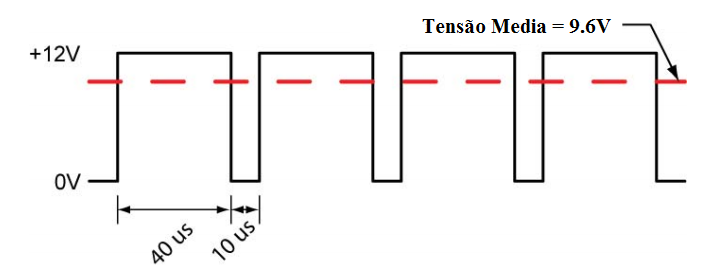
\includegraphics[width=1\textwidth]{figuras/pwm_tensao_media.png}
	\caption{Tensão média produzida por um sinal PWM}
	\fonte{ \citeonline{mecaweb2019}}
	\label{fig:avervoltagepwm}
\end{figure}

\begin{comment}
%Modelo de inclusão de equação. É só copiar, tomar como modelo e modificar.
\begin{equation}
{u_r} = \sqrt {{u^2} + {{(\dot \theta R)}^2} + 2u(\dot \theta R)\cos \theta }
\label{eq:Vrelativa}
\end{equation}

\begin{equation}
\beta  = \arctan \left( {\frac{{\dot \theta Rsen\theta }}{{u + \dot \theta R\cos \theta }}} \right)
\label{eq:beta}
\end{equation}

\begin{equation}
\alpha  = \left| {\frac{{\pi  + \beta  - \theta }}{{2\pi }}} \right| - \pi
\label{eq:alfa}
\end{equation}

Uma vez que o angulo de ataque é conhecido os coeficiente de sustentação ($C_L$) e arrasto ($C_D$) podem ser obtidos. Assim as forças de sustentação ($L$) e arrasto ($D$) podem ser calculadas conforme \autoref{eq:L} e \autoref{eq:D}, respectivamente. Sendo $\rho$ a massa específica do fluido, $c$ a corda, ....

\begin{equation}
L = \frac{1}{2}\rho cu_r^2{C_L}
\label{eq:L}
\end{equation}

\begin{equation}
D = \frac{1}{2}\rho cu_r^2{C_D}
\label{eq:D}
\end{equation}


\section{Modelagem dinâmica}
\label{sec:modelagemdinamica}
\end{comment}